\documentclass{beamer}

\usepackage[utf8]{inputenc}
\usecolortheme{beaver}
\usepackage{caption}
\usepackage{subcaption}
\usepackage{mathtools}
\usepackage{todonotes}
\usepackage{amsmath}
\usepackage{bm}
\usepackage{listings}
\usepackage{ragged2e}
\usepackage{titlecaps}
\usepackage{fancyvrb}

\def\ci{\perp\!\!\!\!\!\perp}

\newtheorem{proposition}{Proposition}
\Addlcwords{for a is but and with of in as the etc on to if}

\setbeamertemplate{section in toc}{\inserttocsectionnumber.~\inserttocsection}
\usetheme{Boadilla}
\makeatletter
\setbeamertemplate{footline}{%
    \leavevmode%
    \hbox{%
        \begin{beamercolorbox}[wd=.3\paperwidth,ht=2.25ex,dp=1ex,center]{author in head/foot}%
            \usebeamerfont{author in head/foot}\insertshortauthor\expandafter\beamer@ifempty\expandafter{\beamer@shortinstitute}{}{~~(\insertshortinstitute)}
        \end{beamercolorbox}%
        \begin{beamercolorbox}[wd=.55\paperwidth,ht=2.25ex,dp=1ex,center]{title in head/foot}%
            \usebeamerfont{title in head/foot}\insertshorttitle
        \end{beamercolorbox}%
        \begin{beamercolorbox}[wd=.15\paperwidth,ht=2.25ex,dp=1ex,right]{date in head/foot}%
            \usebeamerfont{date in head/foot}\insertshortdate{}\hspace*{2em}
            \insertframenumber{} / \inserttotalframenumber\hspace*{2ex} 
        \end{beamercolorbox}}%
        \vskip0pt%
    }
\makeatother

\begin{document}

\title[]{Statistical and Causal Robustness for Causal Null Hypothesis Tests}
\date{}

\maketitle

\begin{frame}{Background}
	\begin{figure}
		\center
		\includegraphics[page=1]{figures.pdf}
		\caption*{Workflow for estimating causal effect from observational data}
	\end{figure}

	\vspace{1em}
	\begin{itemize}
		\item Difficult to construct DAG from data.
		\item Typically done by hand based on domain knowledge.
		\item Different structure learning algorithms are available.
		\item No easy way to test whether the DAG is correct.
	\end{itemize}	
\end{frame}

\begin{frame}{Background}
	\begin{figure}
		\center
		\includegraphics[page=2]{figures.pdf}
	\end{figure}
	\vspace{1em}
	\begin{itemize}
		\item Given a DAG, check whether parameter is estimable.
			\begin{figure}
				\center
				\begin{subfigure}{0.25 \textwidth}
					\center
					\includegraphics[page=4, scale=0.8]{figures.pdf}
				\end{subfigure}%
				\begin{subfigure}{0.25 \textwidth}
					\center
					\includegraphics[page=5, scale=0.8]{figures.pdf}
				\end{subfigure}
			\end{figure}
		\item do-calculus gives a complete solution but difficult to apply in practice.
		\item Special case solutions: Backdoor, Front-door, Instrumental Variables (IV).
		\item Each criterion makes different assumptions about the specified model.
		\item Assumptions are difficult to test in data.
	\end{itemize}
\end{frame}

\begin{frame}{Background}
	\begin{figure}
		\center
		\includegraphics[page=3]{figures.pdf}
	\end{figure}
	\vspace{1em}
	\begin{itemize}
		\item If the model is correctly specified, and identification criterion assumptions are satisfied, an estimator can be used.
		\item The estimator makes further assumptions about the data such as linearity, distribution, etc.
		\item Statistically robust estimators are available, i.e. unbiased, fast convergence, etc.
	\end{itemize}
\end{frame}

\begin{frame}{Example}
	\begin{itemize}
		\item Test whether there is an effect of \textbf{smoking} on \textbf{glucose levels}.
		\item Given a dataset $ D = \{ C, Z, A, M, Y \} $.
			\begin{itemize}
				\item Treatment ($ A $): Smoking status.
				\item Outcome ($ Y $): Glucose level.
				\item Baseline covariates ($ C $): Age, sex, BMI, past history of heart disease, and past glucose level.
				\item Mediator ($ M $): Hypertension.
				\item IV ($ Z $): Past hypertension.
			\end{itemize}
		\item Estimate the average causal effect (ACE) of smoking on glucose.
	\end{itemize}
			$$ \beta = \mathbb{E}[Y(A=1)] - \mathbb{E}[Y(A=0)] $$
\end{frame}

\begin{frame}{Example}
	\begin{figure}
		\center
		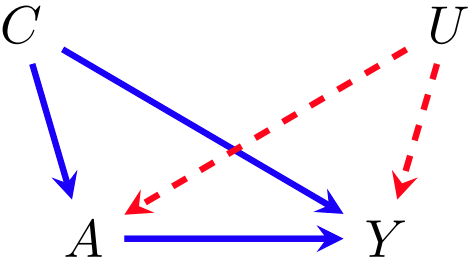
\includegraphics[scale=0.2]{m1.png}
	\end{figure}
	\vspace{1em}
	\begin{itemize}
		\item Backdoor criterion can identify $ A \rightarrow Y $.
		\item Identificaiton assumption: No unobserved confounding.
		\item A potential unobserved confounder could be health consciousness.
		\item If identificaiton assumptions are satisfied, estimator:
		\begin{equation*}
				\begin{split}
					\beta &= \mathbb{E}[\mu(1, C) - \mu(0, C)] \\
					\mu(a, c) &= \mathbb{E}(Y | A=a, C=c)
				\end{split}
			\end{equation*}

	\end{itemize}
\end{frame}

\begin{frame}{Example}
	\begin{figure}
		\center
		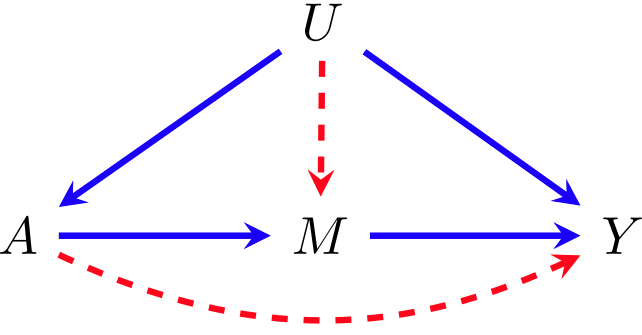
\includegraphics[scale=0.2]{m2.png}
	\end{figure}
	\begin{itemize}
		\item Front-door model can identify $ A \rightarrow Y $.
		\item Identification criterion:
			\begin{itemize}
				\item Allows unobserved confounding between the treatment and outcome.
				\item Treatment effect should only go through mediator.
				\item No effect of unobserved confounding on the mediator.
			\end{itemize}
		\item If identification assumptions are satisfied, estimator:
			\begin{equation*}
				\begin{split}
					\beta &= \mathbb{E}[\mathbb{E}[\gamma(M, C) | A = 1, C] - \mathbb{E}[\gamma(M, C) | A =0, C]] \\
					\gamma(m, c) &= \mathbb{E}[\mu(m, A, c) | C=c] \\
					\mu(m, a, c) &= \mathbb{E}(Y | M=m, A=a, C=c)
				\end{split}
			\end{equation*}
	\end{itemize}
\end{frame}

\begin{frame}{Example}
	\begin{figure}
		\center
		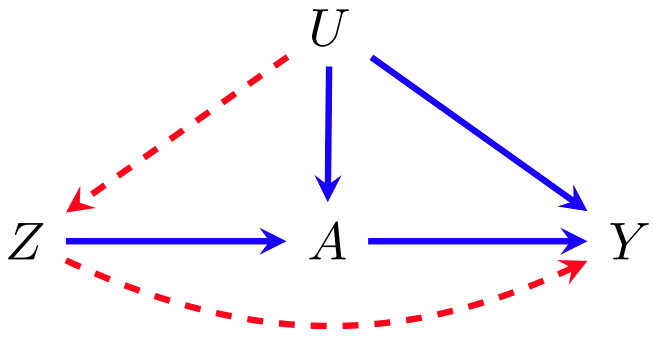
\includegraphics[scale=0.2]{m3.png}
	\end{figure}
	\vspace{1em}
	\begin{itemize}
		\item Instrumental Variable can be used for identification. $ Z $ is the IV.
		\item Identificaiton assumption: $ Z $ should be correlated with $ Y $ only through $ A $.
		\item If identification condition is satisfied, estimator:
			$$ \beta = \frac{\mathbb{E}(Y | Z = 1) - \mathbb{E}(Y | Z = 0)}{\mathbb{E}(A | Z = 1) - \mathbb{E}(A | Z=0)} $$
	\end{itemize}
\end{frame}

\begin{frame}{Proposed Solution: Overview}
	\begin{itemize}
		\item Focus only on whether causal effect is present (not estimation).
		\item Develop a statistical test to test whether causal effect is present. 
			$$ H_0: \beta = 0 $$
		\item As specifing a single correct model is difficult, test a set of models.
		\item The statistical test works if even one of the models is correct.
		% \item It is challenging to come up with a single correct specification of the model.
		% \item Instead, use a bunch of different model. And the paper proposes a robustness test on this set of models.
		% \item The test check if the causal assumption is true if atleast one of the specified model is correct.
		% \item They use something called Evidence Factors to combine the results from testing on the models.
		% \item Limited to semi-parameteric estimation methods. For convergence properties of the test??
	\end{itemize}
\end{frame}

\begin{frame}{Test Development}
	\begin{itemize}
		\item $H_{0}: \beta = 0 $
		\item IID data $ O_1, \cdots, O_n $ from unknown distribution $ P $.
		\item Considering $ K > 1 $ causal models $ M_1, \cdots, M_k $.
		\item $ \psi_{k, P} $ is the identifying function for $ \beta $ under $ M_k $.
	\end{itemize}

	\vspace{2em}

	Under null, if at least one of the models is correct, at least one of $ \psi_{k, P} = 0 $.
	$$ H_0: \prod_{k=1}^{K} \psi_{k, P} = 0 $$
\end{frame}

\begin{frame}{Test Development: Assumptions}
	\begin{itemize}
		\item Linear estimators $ \psi_{k, n} $ for $ \psi_{k, P} $.
		\item Estimators have influence functions $ \Phi_{k, P} $ under statistical conditions $ C_k $.
		\item \begin{equation*} 
				\begin{split}
					\psi_{k, n} - \psi_{k, P} &= \mathbb{P}_n \Phi_{k, P} + O_{P}(n^{-1/2}) \\
					\mathbb{P}_n f &= \frac{1}{n} \sum_{i=1}^{n} f(O_i) \\
				\end{split}
		      \end{equation*}
		\item Statistical conditions $ C_k$ include convergence and complexity constraints for nuisance estimators.
	\end{itemize}
\end{frame}

\begin{frame}{Test Development: Asymptotic Distribution}
\end{frame}

\begin{frame}{Test Development: Calibration}
	\begin{figure}
		\center
		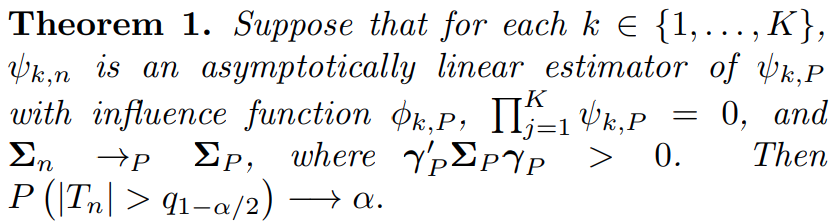
\includegraphics[scale=0.3]{theorem1.png}
	\end{figure}
\end{frame}

\begin{frame}{Test Development: Power}
	\begin{figure}
		\center
		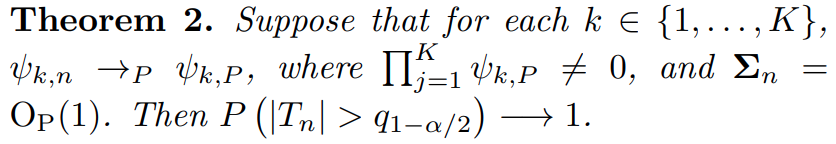
\includegraphics[scale=0.3]{theorem2.png}
	\end{figure}
\end{frame}

\begin{frame}{Empirical Analysis: Setup}
	\begin{figure}
		\begin{subfigure}{0.33 \textwidth}
			\center
			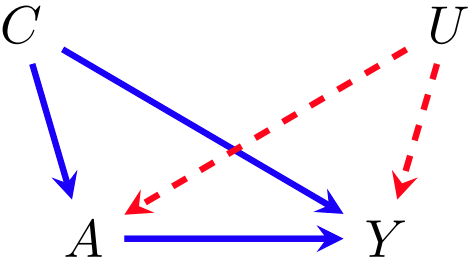
\includegraphics[scale=0.15]{m1.png}
		\end{subfigure}%
		\begin{subfigure}{0.33 \textwidth}
			\center
			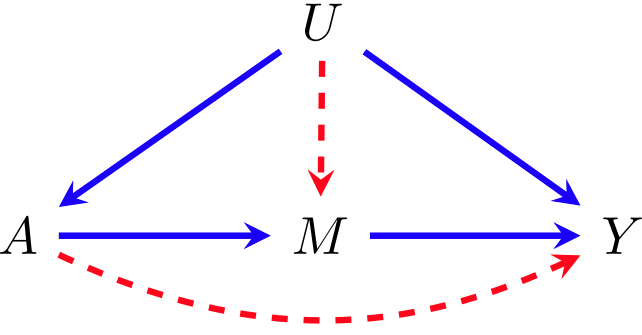
\includegraphics[scale=0.15]{m2.png}
		\end{subfigure}%
		\begin{subfigure}{0.33 \textwidth}
			\center
			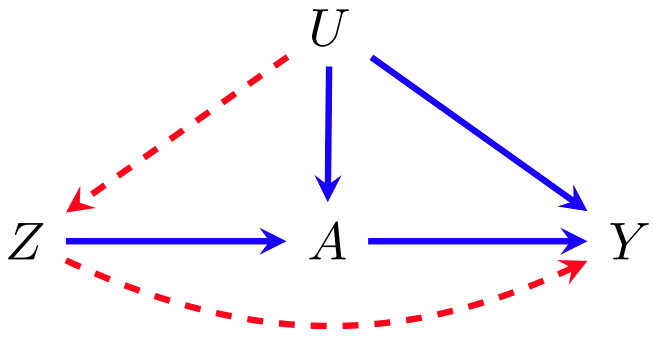
\includegraphics[scale=0.15]{m3.png}
		\end{subfigure}
	\end{figure}

	\begin{itemize}
		\item Use the model with blue edges for the test.
		\item Generate data under model violations (red edges).
		\item Test with either $1$, $2$, or $3$ model violations.
		\item To generate violations from both $M_1$ and $M_2$ introduce a direct effect from $ Z $ to $ Y $.
	\end{itemize}
\end{frame}

\begin{frame}{Empirical Analysis: Calibration}
	\begin{figure}
		\center
		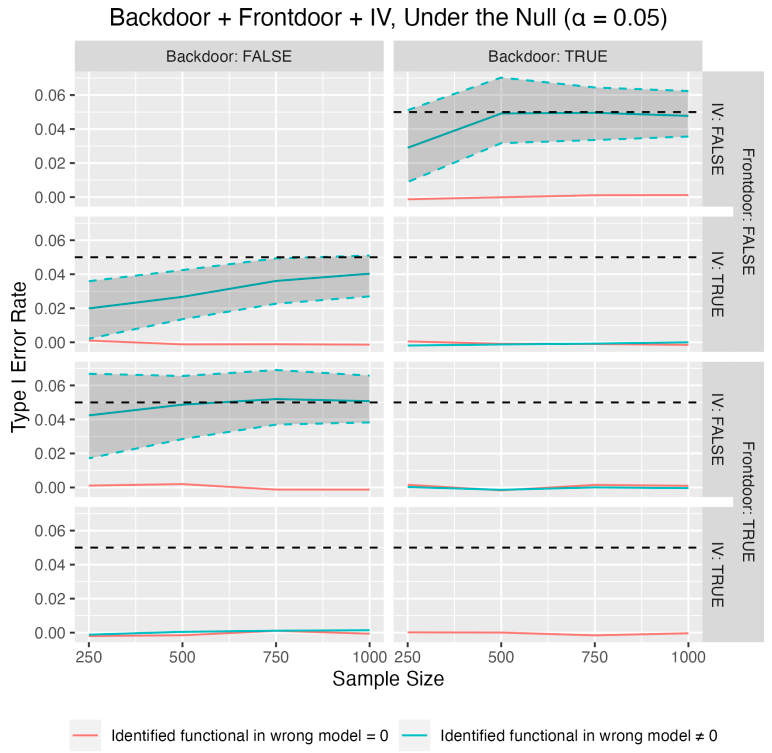
\includegraphics[scale=0.3]{calibration.png}
	\end{figure}
\end{frame}

\begin{frame}{Empirical Analysis: Power}
	\begin{figure}
		\center
		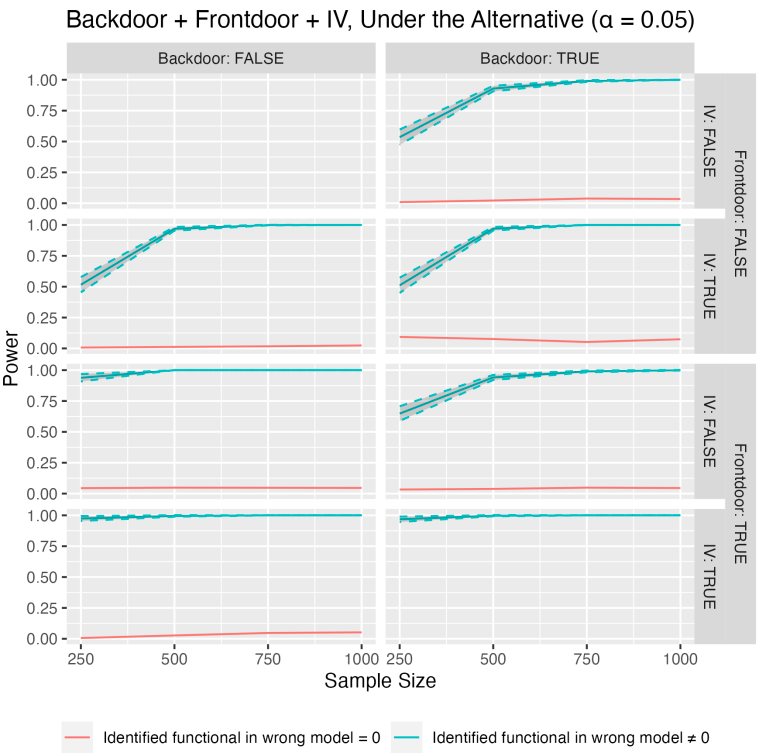
\includegraphics[scale=0.3]{power.png}
	\end{figure}
\end{frame}

\begin{frame}{Empirical Analysis: Setup}
	\begin{figure}
		\center
		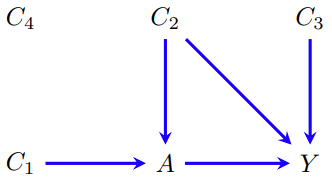
\includegraphics[scale=0.3]{empirical_dag.png}
	\end{figure}
	\begin{itemize}
		\item All three models considered are backdoor models.
		\item The adjustment sets considered are different. 1) $ \{ C_1, C_2, C_3, C_4 \} $, 2) $ \{ C_1, C_3 \} $, and 3) $ \{ C_1, C_4 \} $.
		\item First model is correct, the other two are incorrect.
	\end{itemize}
\end{frame}

\begin{frame}{Empirical Analysis: Multi Backdoor}
	\begin{figure}
		\center
		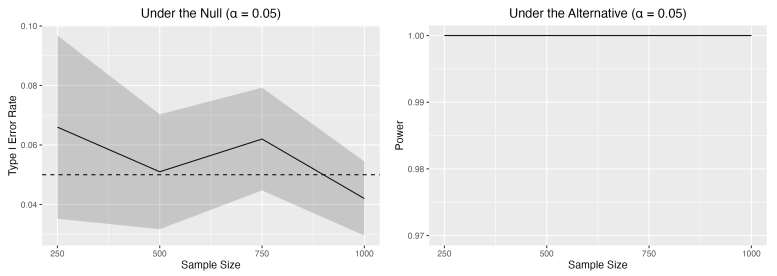
\includegraphics[scale=0.45]{multi_back.png}
	\end{figure}
\end{frame}

\begin{frame}{Real Data Example}
	\begin{figure}
		\center
		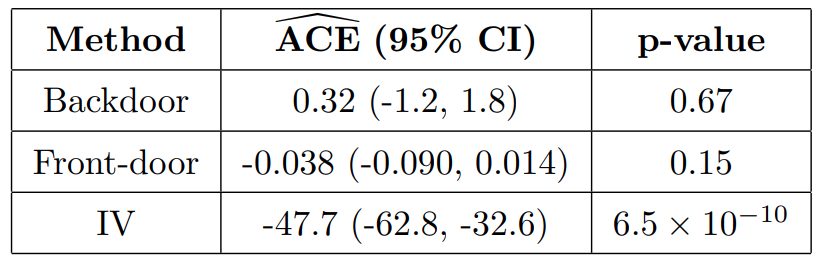
\includegraphics[scale=0.2]{table.png}
		\caption*{Estimated effect using the models.}
	\end{figure}

	The proposed method returns a p-value of 0.68 failing to reject the null hypothesis.
\end{frame}

\begin{frame}{Conclusion}
	\begin{itemize}
		\item A valid test if at least one of hte proposed causal models is correct, without knowing which one is correct.
		\item 
	\end{itemize}
\end{frame}

\end{document}
